\documentclass[11pt,a4paper]{report}

\usepackage[nottoc]{tocbibind} % controls table of contents, nottoc means not-table of contents i.e. exclude "Contents" itself from contents

%\usepackage{epsfig}
%\usepackage{siunitx}
\usepackage{amsmath, amsfonts, amssymb, makeidx, lmodern, float, csquotes, caption, subcaption, array, tabularx, enumerate, multirow}

\usepackage{soul}

\usepackage{fontspec}
\usepackage{polyglossia}

\setdefaultlanguage{english}
\setotherlanguage{sanskrit}

\newfontfamily\devanagarifont[
Script=Devanagari
]{Noto Serif Devanagari}

\usepackage[left=2.5cm,right=2.5cm,top=2.5cm,bottom=2.5cm]{geometry}

\usepackage[usenames, dvipsnames, table]{xcolor}
\definecolor{myred}{RGB}{120, 0, 0}
\definecolor{mygreen1}{RGB}{234,236,209}
\definecolor{myteal}{RGB}{0,128,128}

\usepackage{graphicx}
\graphicspath{{figures/}}

\usepackage[backend=biber, sorting=none, %
            defernumbers=true, style=nature, doi=true]{biblatex}

\addbibresource{references.bib}

\usepackage{hyperref}
\hypersetup{colorlinks=true, linkcolor=blue, citecolor=blue, urlcolor=blue}

\usepackage{titling}
\setlength{\droptitle}{-3.5cm}

\usepackage{titlesec}

\titleformat{\chapter}[display]
{\normalfont\huge\bfseries}
{Chapter \thechapter}
{0pt}
{\Huge}

\titlespacing*{\chapter}
{0pt}
{-20pt}
{30pt}

\newcounter{Section*}
\newcommand\addtotoc[1]{
	\refstepcounter{Section*}
	\addcontentsline{toc}{section}{#1}}

\setlength{\parindent}{4em}
\setlength{\parskip}{0.1em}
\renewcommand{\baselinestretch}{1.5}

\newcommand{\bs}[1]{\boldsymbol{#1}}

\setlength{\fboxsep}{2pt}

\newcommand{\ghl}[1]{%
\colorbox{green}{#1}
}

\def\session{\ifcase\month\or
	January\or February\or March\or April\or May\or June\or
	July\or August\or September\or October\or November\or December\fi
	,\space \number\year}

%\title{\centering\LARGE \bf Neural Network Stochastic Differential Equation Models for Financial Data Forecasting }
\title{
	\LARGE\bfseries
	Neural Network Stochastic Differential Equation Models for Financial Data Forecasting
}
\author{

\includegraphics[height=4cm, scale=1]{figures/bhu1.png}\\[10pt]
    \Large A project submitted\\
    \Large for partial fulfillment of the requirements for the award of the degree of\\
    \Large Master of Science\\[4ex]
    \Large \textit{by}\\[0.5ex]
	\LARGE \bf Ananda Biswas\\[12pt]
	\large M.Sc. in Statistics \& Computing\\
	\large Exam Roll No.: 24419STC053 \\[4ex]
	\Large \textit{Under the supervision of}\\
	\LARGE Dr. Ganga Ram\\
    \Large DST-CIMS, BHU\\[10ex]
	\LARGE \bf Centre for Interdisciplinary Mathematical Sciences\\
	\LARGE \bf I.Sc., Banaras Hindu University\\
	\LARGE  Varanasi, India-221005\\[4em]
	\noindent\begin{minipage}{0.5\textwidth}
		\large \textbf{Enrollment No: 482721}
	\end{minipage}%
	\begin{minipage}{0.5\textwidth}
		\raggedleft \large \session
	\end{minipage}
}
\date{}

\begin{document}

\begingroup
\let\clearpage\relax
\pagenumbering{gobble}
\maketitle
\endgroup


\pagenumbering{roman}
%%--------Declaration of Authorship---------%%
%\addtotoc*{Declaration of Authorship}
\vspace{3em}
\section*{\centering \huge Declaration}
\vspace{3em}
\begin{large}
	I, \textbf{Ananda Biswas}, hereby declare that the project titled \emph{\textbf{Neural Network Stochastic Differential Equation Models for Financial Data Forecasting}} and the work presented therein are my own and original, carried out under the supervision of \textbf{Dr. Ganga Ram, DST-CIMS}, Banaras Hindu University, during the period from March 2026 to May 2026. This project has been submitted to the DST-Centre for Interdisciplinary Mathematical Sciences, Banaras Hindu University, in partial fulfilment of the requirements for the M.Sc. in Statistics $\&$ Computing course. To the best of my knowledge and belief, the information and data presented in this project are authentic. This work has not been submitted to any other university or institution for the award of any degree, diploma, or fellowship, nor has it been published previously.
	
	\vspace{5em}
\begin{flushright}
	\rule[.1em]{12em}{1pt}\\
	\textbf{Place:} \hfill \textbf{ANANDA BISWAS}\\
	\textbf{Date:}\hfill \textbf{24419STC053}
\end{flushright}
\clearpage
\end{large}

\newpage


%%-------Approval by supervisor------%%
%\begin{figure}[t]
	%\centering
	%
\includegraphics[width=10cm, height=3cm]{figures/BHU.png}
%\end{figure}
%{\color{myred}
	%\Large \bfseries \centering DST-CIMS, Institute of Science\\
	%\Large \bfseries \centering Banaras Hindu University, Varanasi\\}
%\begin{flushleft}
%	\color{myred}
%	\rule[.1em]{\textwidth}{1pt}
%\end{flushleft}
\vspace*{3em}
\section*{\centering \Large \textit{CERTIFICATE}}
\vspace{3em}
\hspace*{1cm}This is to certify that \textbf{[Insert Your Name Here]}, a student of the \textbf{Master of Science in Statistics \& Computing}, Semester IV of the \textbf{DST-Centre for Interdisciplinary Mathematical Sciences}, Institute of Science, Banaras Hindu University, bearing exam roll no. \textbf{[XXXXXSTCXXX]} and enrollment no. \textbf{[XXXXXX]} of 2024-2026 has successfully completed his  project entitled ``\textbf{[Insert Project Title Here]}". The project was completed under my direct supervision and guidance for the partial fulfillment of the course curriculum of Master of Science in Statistics \& Computing. He carried out the whole work with utmost sincerity, and the present report is the outcome of his sincere efforts and endeavors. This work either in the present form or in part in any other form is not being submitted anywhere to the best of my knowledge.

%The project was done from March 2024 to May 2024 in our centre. During this period, he was fully involved in this project and subject.
\vspace*{5em}
\begin{center}
\begin{tabularx}{\linewidth}{XXX}
    & & \centering\rule[.1em]{11em}{1pt} \tabularnewline
    & & \centering Supervisor \tabularnewline
\end{tabularx}
\vspace{5em}

\begin{tabularx}{\linewidth}{XXX}
    \centering\rule[.1em]{11em}{1pt} & & \centering\rule[.1em]{11em}{1pt} \tabularnewline
    \centering Course Coordinator & & \centering Coordinator, DST-CIMS \tabularnewline
\end{tabularx}
\end{center}
\clearpage

\vspace*{3em}
%\addtotoc{Acknowledgment}
\section*{\centering \huge \textit{Acknowledgment}}
\vspace{3em}
I am honoured to have this opportunity to convey my sincere gratitude to my supervisor, \textbf{Dr. Ganga Ram}, for his precious supervision, constant motivation, and caring mentorship throughout the tenure of this research. Without his immense knowledge and unparalleled vision, this thesis would not have taken this shape.
\vspace{5em}
\begin{flushright}
	\rule[.1em]{12em}{1pt}\\
	\textbf{Place:} \hfill \textbf{ANANDA BISWAS}\\
	\textbf{Date:}\hfill \textbf{24419STC053}
\end{flushright}
\clearpage
%%-----Dedication-----%%
%\topskip0pt
\vspace*{\fill}

\begin{center}
	\textit{
		{\huge
			To my parents,\\[1em]
			for every sacrifice they made
		}
	}
\end{center}

\vspace*{\fill}

\newpage

\vspace*{\fill}

\begin{center}
	
	{\Large
		\devanagarifont
		ॐ
		
		\vspace{0.7cm}
		
		{\Large
			\devanagarifont
			सरस्वति महाभागे विद्ये कमललोचने ।\\[0.5cm]
			विद्यारूपे विशालाक्षि विद्यां देहि नमोऽस्तुते ॥
		}
	}
	
\end{center}

\vspace*{\fill}

\newpage

\addtotoc{Abstract}
\section*{\centering \huge \textit{Abstract}}
    This study employs a collection of stochastic differential equations with drift and diffusion coefficients approximated by neural networks for financial time series forecasting. In particular, the performance of Stochastic Differential Equation Network with Brownian Motion and Lévy induced Stochastic Differential Equation Network with varying $\alpha$ are deployed on two major stock market indices : NIFTY50, India and SSE50, China. The models are employed to forecast index movement across multiple prediction horizons of $1, 3, 7, 14$ days ahead, enabling both immediate and long-term prediction capabilities. The models aim to capture the stochastic and non-linear dynamics inherent in financial data through differential equation driven neural architectures. The findings suggest that stochastic differential equation based neural networks like SDENet, LDENet provide a promising approach for modelling highly volatile financial data with improved predictive performance. 
\clearpage


\tableofcontents

\newpage
\listoffigures

\newpage
\listoftables



\clearpage

\pagenumbering{arabic}
\input{Sections/10_Introduction}
\section{Problem Statement}

Financial markets are highly volatile and uncertain systems influenced by numerous economic, political and social factors. Due to the presence of irregular fluctuations, abrupt jumps and nonlinear dependencies, accurately forecasting stock market indices remains a difficult challenge in time series analysis. Traditional statistical approaches such as autoregressive and moving average models generally rely on assumptions of linearity and Gaussian noise, which limit their effectiveness when dealing with real world financial data exhibiting heavy tailed distributions and sudden transitions.

Recent advances in deep learning have improved the capability of predictive models by enabling the extraction of complex nonlinear patterns from sequential data. However, many conventional deep learning architectures are deterministic in nature and may fail to adequately represent the stochastic behaviour inherent in financial systems. Stochastic differential equation based neural networks provide a promising alternative by modeling the hidden dynamics of neural networks through continuous stochastic processes. In particular, SDE-Net incorporates Brownian motion to represent uncertainty in the evolution of hidden states.

Although Brownian motion based models are effective in capturing continuous random fluctuations, they may not sufficiently describe discontinuous jumps frequently observed in stock market behaviour. Financial time series often contain extreme events such as sudden crashes or rapid price surges, indicating the presence of non-Gaussian characteristics. Lévy processes, which generalize Brownian motion by allowing jump discontinuities, may therefore provide a more realistic stochastic framework for modeling such phenomena.

The primary objective of this project is to investigate whether Lévy driven neural differential equation models can improve forecasting performance over traditional Brownian motion driven SDE-Net models. Using real financial datasets from the NIFTY50 and SSE50 indices, the project aims to compare the predictive capabilities of these stochastic neural architectures under multiple forecasting horizons. The study further seeks to analyze the effectiveness of different stochastic perturbations in capturing the complex and uncertain dynamics of financial markets.

\clearpage
\chapter{Data Description}

The datasets used in this project consist of historical financial time series data from two major stock market indices, namely the NIFTY50 index of India and the SSE50 index of China. These indices are widely regarded as important indicators of the economic and financial performance of their respective markets. The NIFTY50 index represents the weighted performance of fifty leading companies listed on the National Stock Exchange of India, while the SSE50 index tracks fifty large scale and highly liquid companies listed on the Shanghai Stock Exchange. Since both indices reflect the behaviour of major financial markets, they provide suitable benchmark datasets for evaluating stochastic forecasting models.

The historical data were collected over multiple years with observations recorded on trading days. Each observation in the datasets originally contained multiple financial attributes including opening price, highest price, lowest price, closing price, trading volume and percentage change for the corresponding trading day. These variables collectively provide different perspectives regarding daily market activity, volatility and trading behaviour. The opening price represents the initial market value at the start of a trading session, while the highest and lowest prices indicate the range of price movement during the day. Trading volume reflects the number of transactions executed, and percentage change measures the relative movement of prices across consecutive trading sessions.

Although the datasets contained several financial indicators, the primary focus of this project was on modeling and forecasting the daily closing prices of the indices. The closing price is commonly regarded as one of the most informative indicators in financial analysis because it summarizes the final market consensus at the end of each trading session. Consequently, the remaining variables such as opening price, highest price, lowest price, volume and percentage change were excluded from the final modeling process. This reduction in dimensionality was performed in order to concentrate specifically on the temporal dynamics of the closing price series and to simplify the learning framework for the stochastic neural differential equation models considered in this study.

Financial time series data generally exhibit non-stationary behaviour characterized by long term trends, volatility clustering, irregular fluctuations and sudden transitions. Such characteristics make financial forecasting particularly challenging because the statistical properties of the data may change over time. Moreover, stock market movements are strongly influenced by external economic conditions, government policies, geopolitical events and investor sentiment, all of which contribute to uncertainty and stochastic behaviour within the series. Due to these complex properties, financial datasets provide an appropriate framework for studying stochastic neural differential equation models which are specifically designed to capture uncertainty and nonlinear temporal dynamics.

Before constructing the forecasting models, the datasets were organized and processed in chronological order to preserve the natural temporal structure of the financial series. Since time series forecasting requires learning from past observations to predict future behaviour, maintaining sequential consistency is essential for realistic modeling. Missing observations and non trading days were handled implicitly through the ordered market records available in the datasets. The resulting financial series therefore represented continuous sequences of historical market behaviour suitable for supervised learning applications.

For the forecasting task, the data were transformed into sequential input-output pairs using sliding window based approaches. In this method, a fixed number of previous observations were utilized as input sequences for predicting future index values. The sliding window framework enables the neural networks to learn temporal dependencies and evolving patterns from historical observations. By continuously shifting the observation window across the dataset, multiple training samples were generated from the same financial series, thereby improving the learning capability of the forecasting models.

In this project, prediction horizons of 1, 3, 7 and 14 days were considered in order to evaluate both short term and relatively longer term forecasting performance. The use of multiple forecasting horizons allows analysis of how predictive accuracy changes as the forecasting interval increases. Short term forecasting generally focuses on capturing immediate market behaviour and local temporal dependencies, whereas longer forecasting horizons involve greater uncertainty and increased difficulty due to the accumulation of stochastic effects over time. Evaluating the models under different horizons therefore provides a more comprehensive understanding of their forecasting capability and robustness.

Normalization techniques were applied to the financial series before feeding them into the neural network models in order to improve numerical stability and facilitate efficient optimization during training. Since raw financial values may vary substantially across different periods and market conditions, normalization helps prevent instability in gradient based learning algorithms and allows the models to converge more effectively. The datasets were subsequently divided into training and testing subsets based on chronological order, ensuring that the temporal dependency structure of the series was preserved. Such a division reflects realistic forecasting conditions in financial applications, where future information remains unavailable during the training phase.

The use of financial datasets from two different markets also allows comparative analysis of the robustness and adaptability of stochastic differential equation based neural networks under varying economic and market conditions. The Indian and Chinese financial markets possess different structural and behavioural characteristics, which may influence the stochastic dynamics present within the data. Since both indices contain complex nonlinear and uncertain patterns, they provide an effective framework for studying the capability of Brownian motion driven SDE-Net models and Lévy driven neural differential equation models in capturing uncertainty and forecasting future market behaviour.
\input{Sections/40_Methods}
\section{Results}

First we preprocess the real data through Phase Space Reconstruction with delay time $\tau = 1$ and embedding dimension $= 30$ and show the prediction accuracy for two different stock trending patterns. In addition, we also numerically analyze the effect of different $\alpha$ values in Lévy motion and forecasting days on prediction accuracy. The
code of all experiments has been open sourced on GitHub : \href{https://github.com/sakunisgithub/python_programming/tree/master/M.Sc.Project}{github.com/sakunisgithub}.

Due to the grave importance of financial market, and its relation to economic development, stock data are the best choice. Two datasets are selected corresponding to NIFTY50 Index of India and SSE50 Index of China \textemdash \, NIFTY50 Index with a total sample size of $4932$ and SSE50 Index with a total sample size of $4917$, both from Jan $2006$ - Mar $2026$.

\begin{figure}[!htbp]
\centering
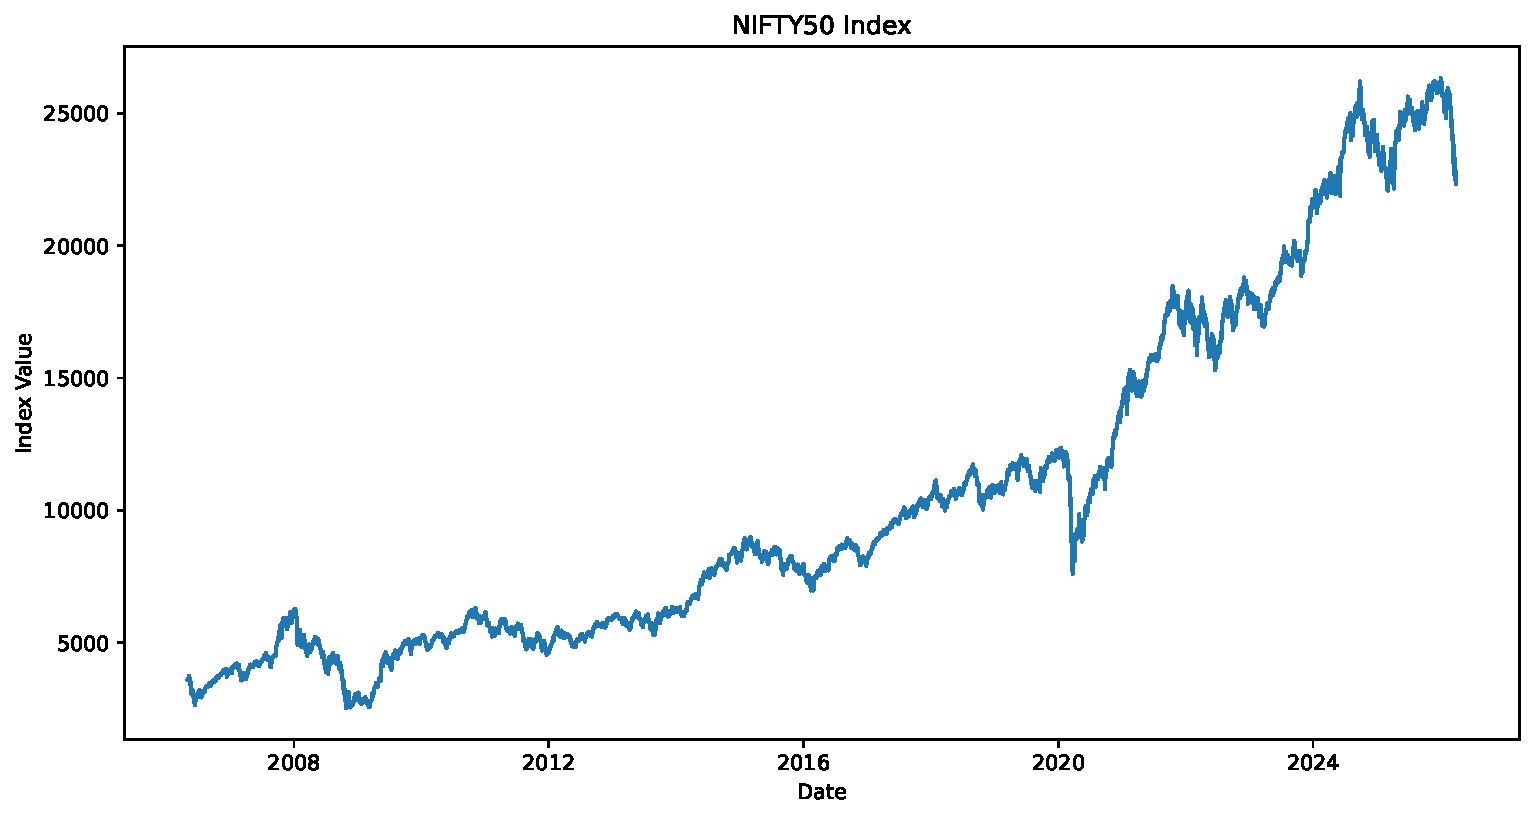
\includegraphics[scale=0.4]{NIFTY50 Index}
\caption{Data set of NIFTY50 Index}
\end{figure}

\begin{figure}
\centering
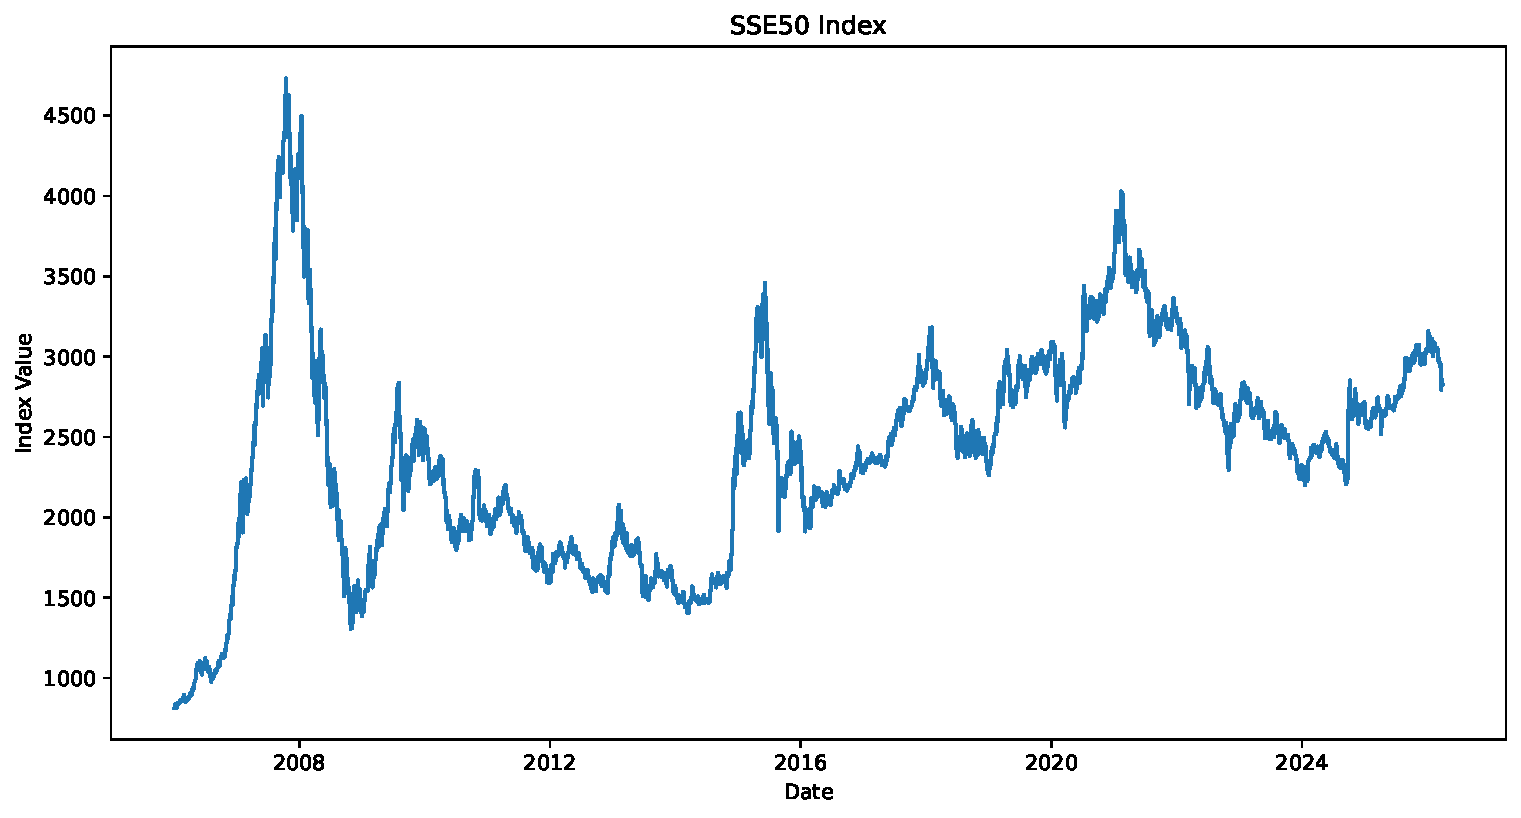
\includegraphics[scale=0.4]{SSE50 Index}
\caption{Data set of SSE50 Index}
\end{figure}

\newpage

For both, data points from $2006$ to $2020$ were taken in training set and $2021$ to $2026$ data points were considered as test set.

\begin{figure}[!htbp]
\centering
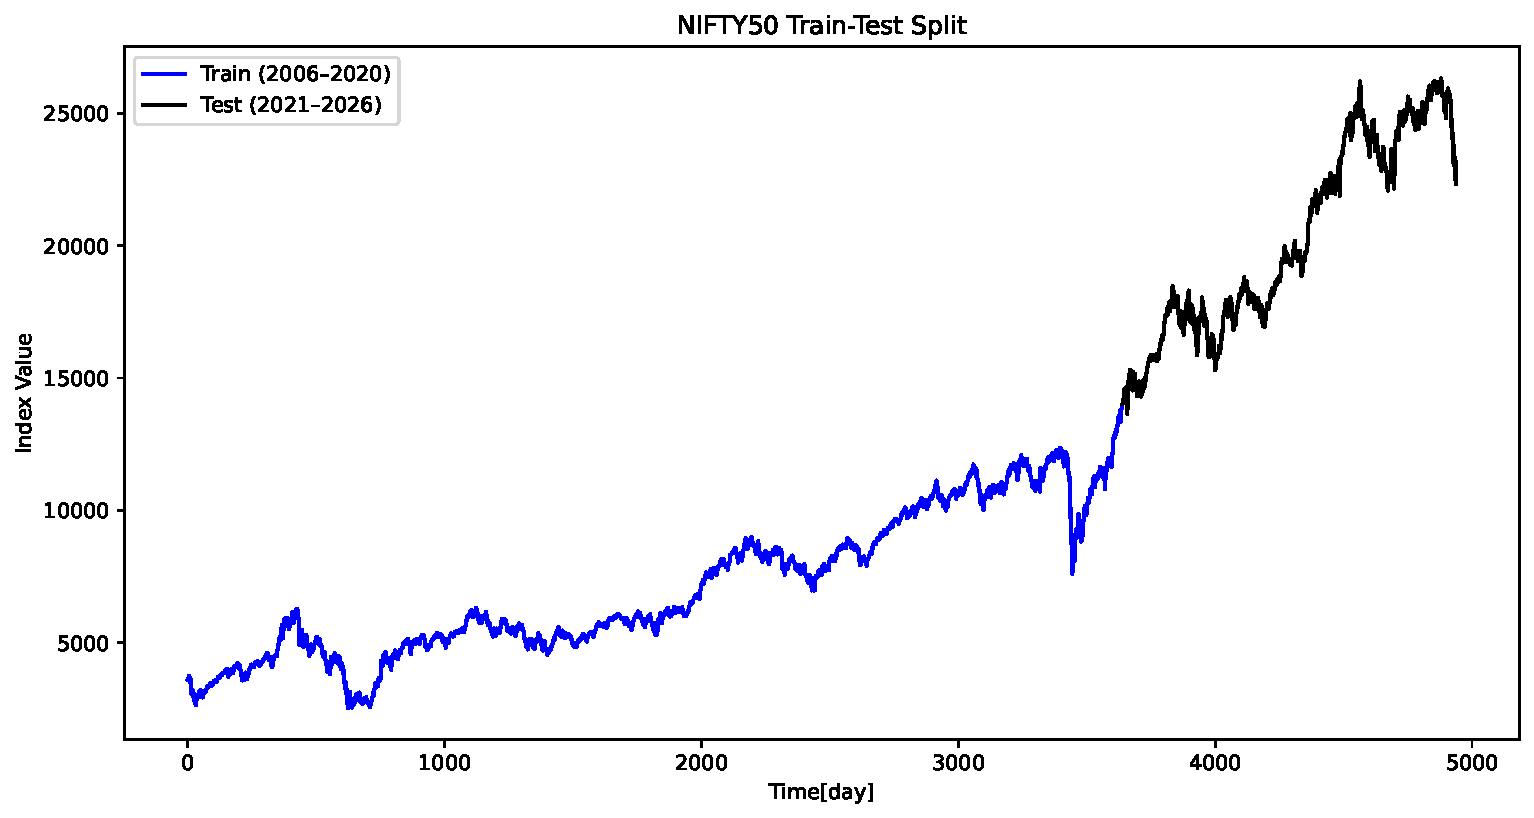
\includegraphics[scale=0.4]{NIFTY50 Train-Test Split}
\caption{Train-Test Split of NIFTY50}
\end{figure}

\begin{figure}[!htbp]
\centering
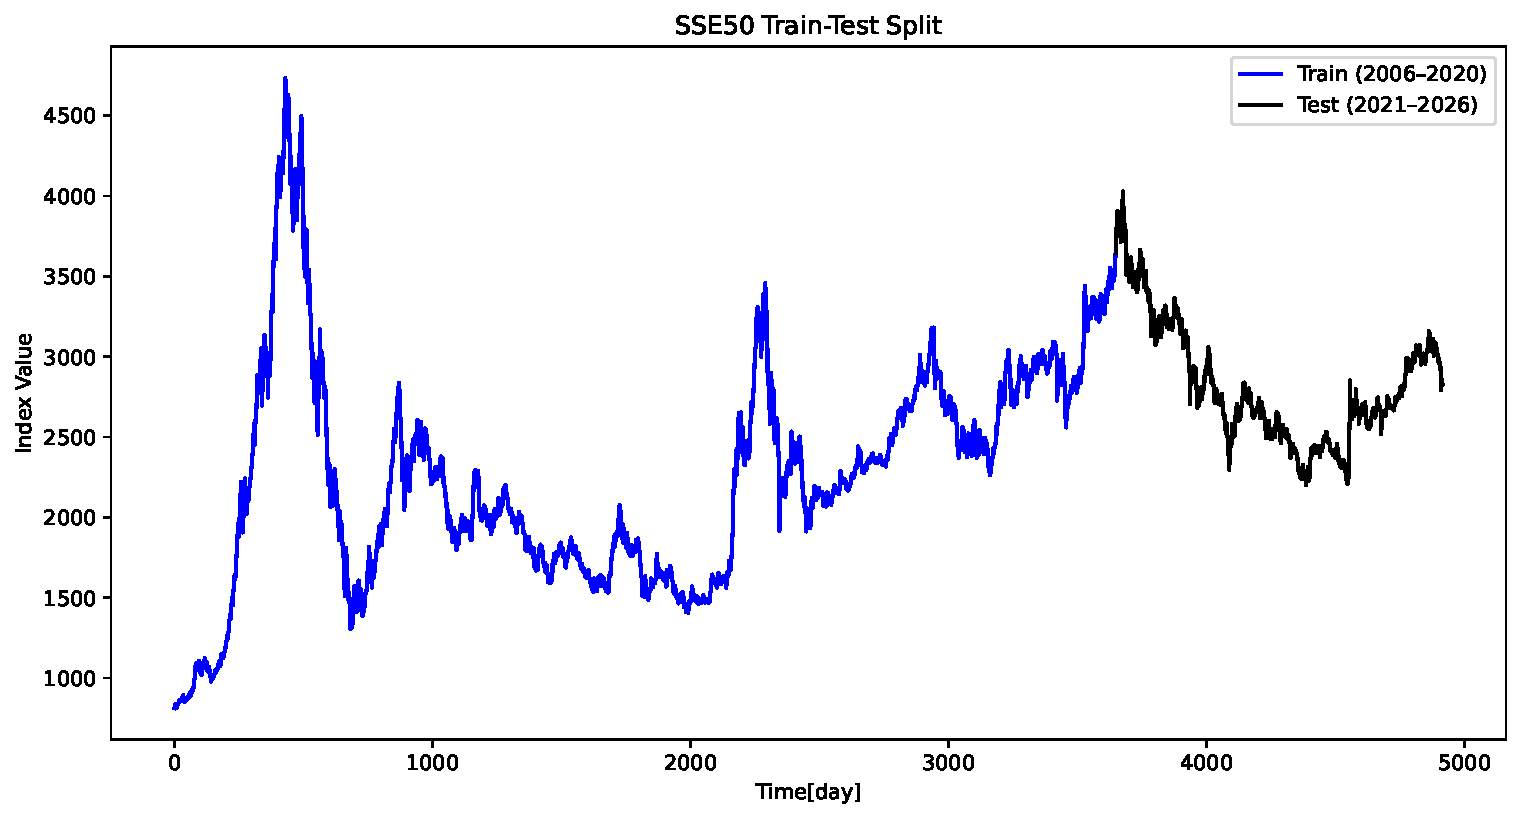
\includegraphics[scale=0.4]{SSE50 Train-Test Split}
\caption{Train-Test Split of SSE50}
\end{figure}

For NIFTY50 Index, training set and test set fluctuations are small. For SSE50 Index, it shows large fluctuations on the training set and relatively small on the test set.

\newpage

\subsection{Forecasting with Different Stock Patterns}

When comparing different stock trend types, we only consider the forecast effect of the first day under the same $\alpha = 1.5$. The results of loss can determine which type of stock data a model is more suitable for.

\begin{figure}[!htbp]
\centering
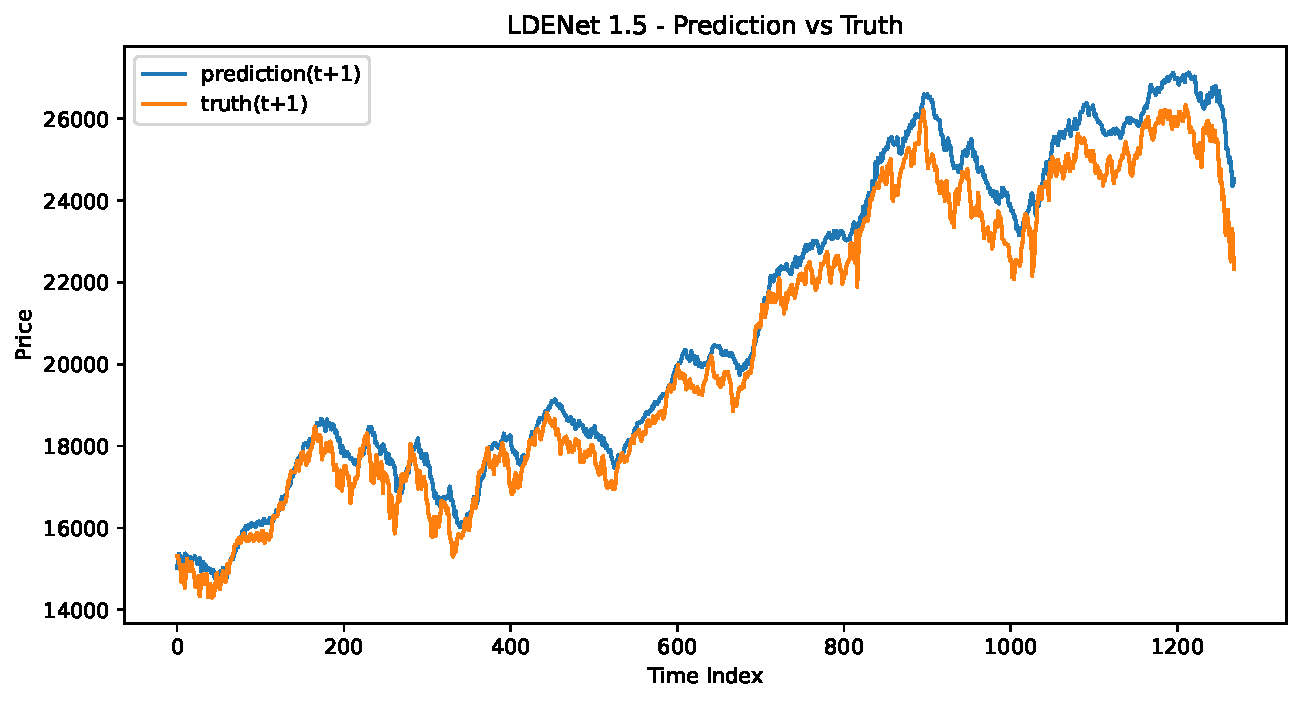
\includegraphics[scale=0.4]{NIFTY50_LDENet_1.5_PH1_Result}
\caption{NIFTY50-First Day Forecast Result}
\label{NIFTY50-First Day Forecast Result}
\end{figure}

\begin{figure}[!htbp]
\centering
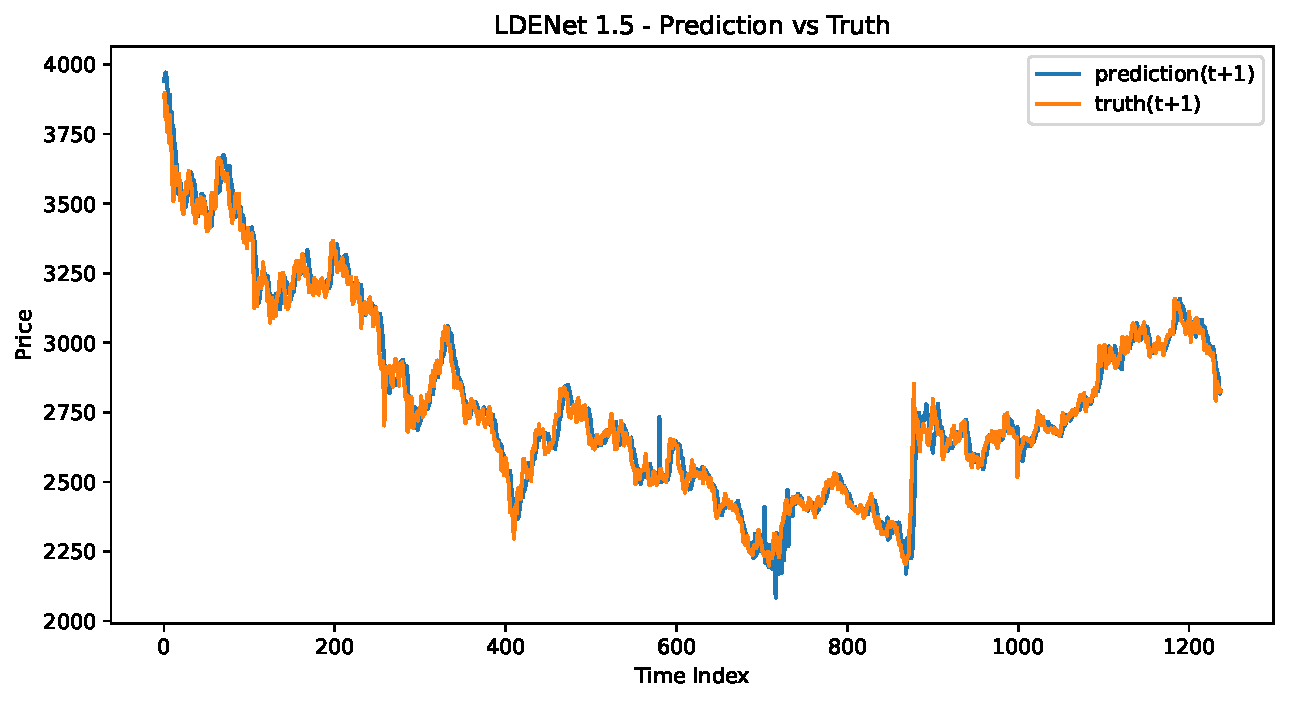
\includegraphics[scale=0.4]{SSE50-LDENet_1.5_PH1_Result}
\caption{SSE50-First Day Forecast Result}
\end{figure}

\begin{table}[!htbp]
\def\arraystretch{1.5}

\begin{center}
\begin{tabular}{>{\centering}m{3cm}>{\centering}m{2cm}>{\centering}m{2cm}>{\centering}m{2cm}>{\centering\arraybackslash}m{2cm}}

\hline

Data & MSE$(t+1)$ & MSE$(t+3)$ & MSE$(t+7)$ & MSE$(t+14)$ \\

\hline
\hline

NIFTY50 Index & $0.07797$ & $0.01815$ & $0.10413$ & $0.16779$ \\

SSE50 Index & $0.00718$ & $0.00896$ & $0.01834$ & $0.02733$ \\

\hline

\end{tabular}
\end{center}
\caption{Forecast Results for Different Stocks $(\alpha = 1.5)$}
\end{table}

It can be seen from Figure (\ref{NIFTY50-First Day Forecast Result}), the prediction of NIFTY50 is poor, but that of SSE50 is praiseworthy. It helps us to comment that the LDE-Net model is suitable for predicting the future value of stocks with large fluctuations in historical data. When the training set fluctuates more frequently with larger amplitude, Lévy noise can better capture the uncertainty in the prediction process,
so as to achieve more accurate prediction. The historical data and test data of NIFTY50 did not have large fluctuations, hence Lévy noise could not give a good fit. In the follow-ups, we shall stick to SDE-Net for NIFTY50 and LDE-Net for SSE50 respectively.

\subsection{Forecasting with Different Models}

We now compare SDE-Net and LDE-Net for different scenarios. As prediction accuracy on first day is highest for either, it is reasonable to compare the effect of forecasting one day.

\begin{figure}[!htbp]
\centering
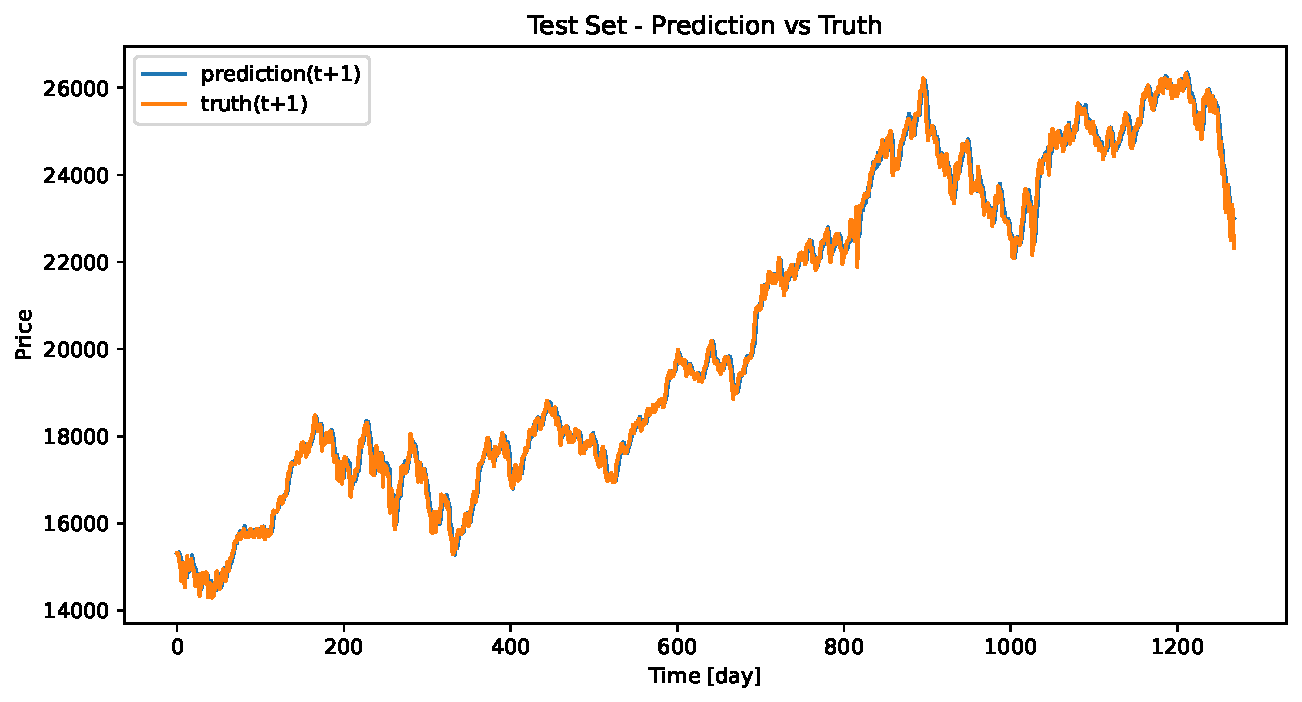
\includegraphics[scale=0.4]{NIFTY50_SDENet_PH1_Result}
\caption{NIFTY50-First Day Forecast Result for SDENet}
\end{figure}

\begin{figure}[!htbp]
\centering
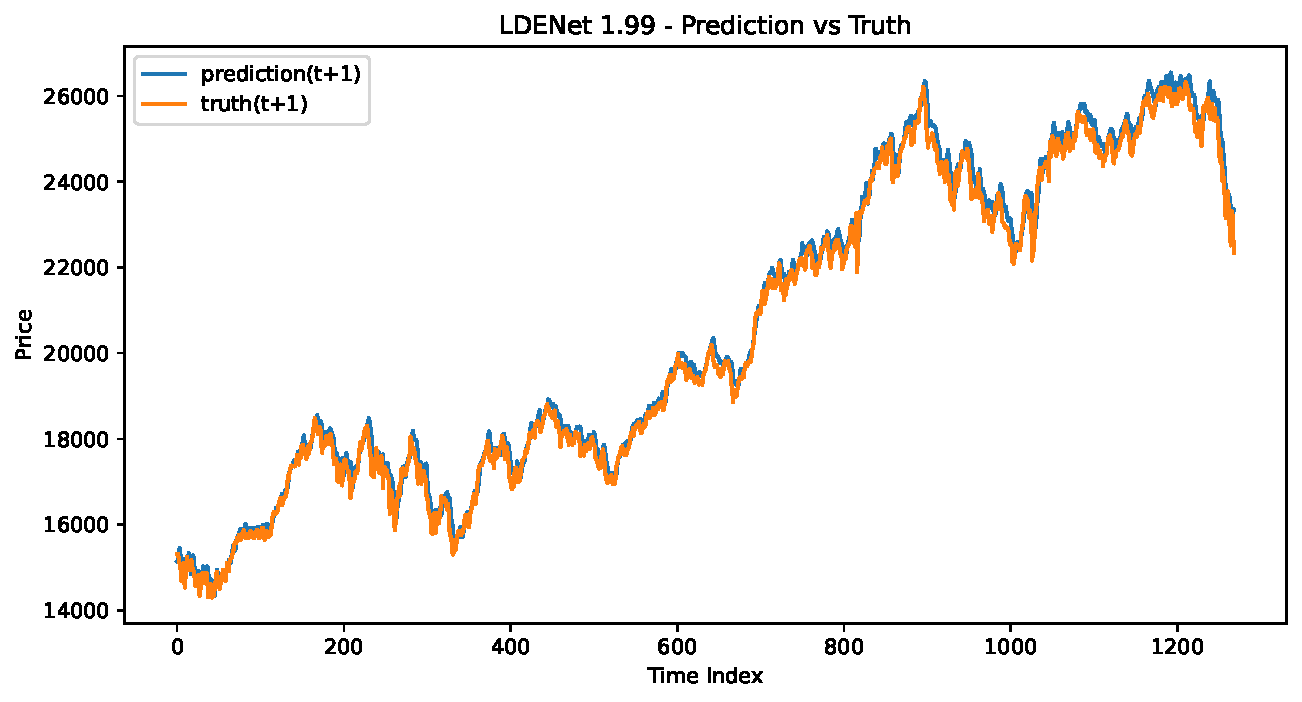
\includegraphics[scale=0.4]{NIFTY50_LDENet_1.99_PH1_Result}
\caption{NIFTY50-First Day Forecast Result for LDENet}
\end{figure}

LDE-Net forecasts seem off as compared to SDE-Net forecasts of NIFTY50 Index values. Now let us have a look at the forecasts for SSE50 Index Values.

\begin{figure}[!htbp]
\centering
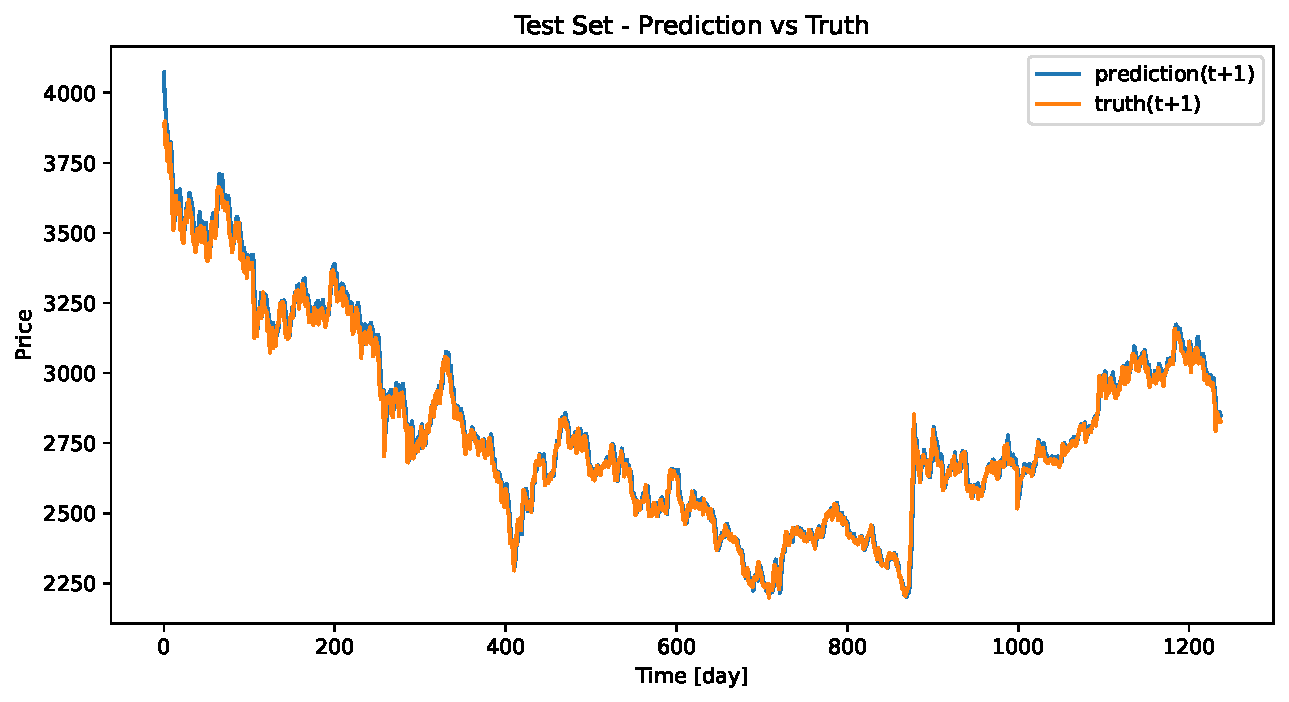
\includegraphics[scale=0.4]{SSE50-SDENet_PH1_Result}
\caption{SSE50-First Day Forecast Result for SDENet}
\end{figure}

\begin{figure}[!htbp]
\centering
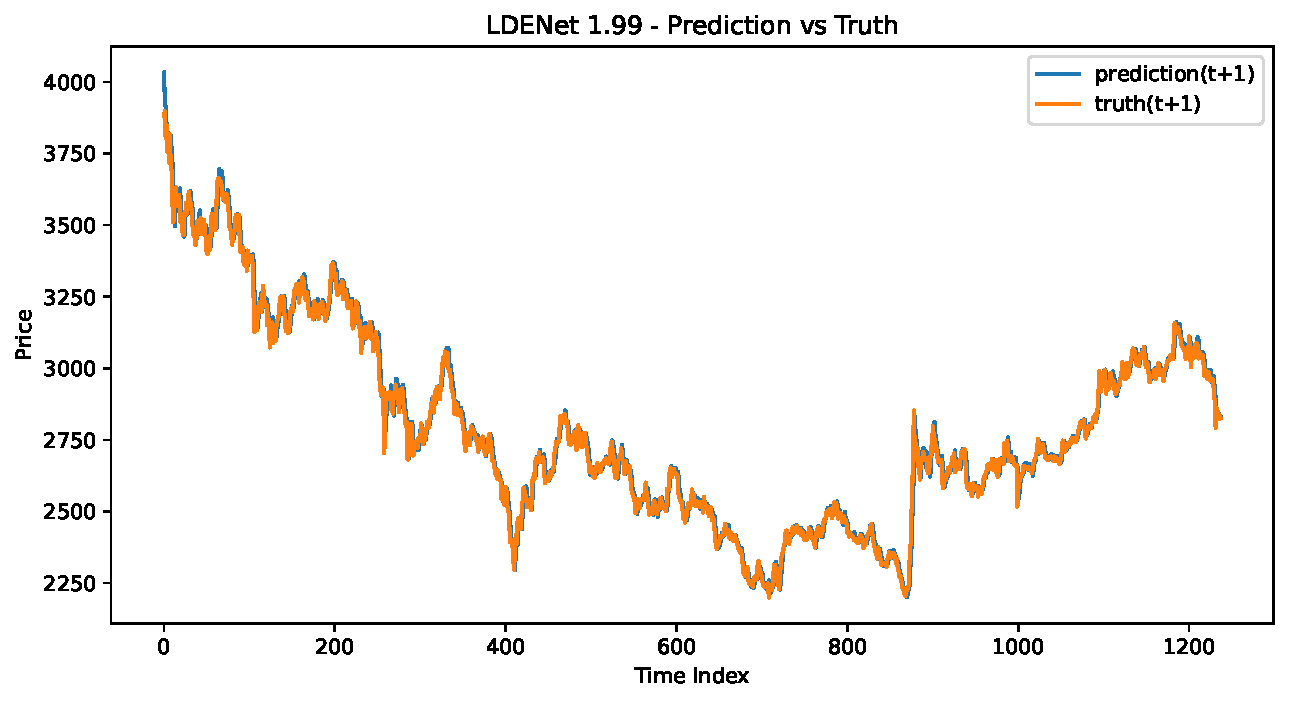
\includegraphics[scale=0.4]{SSE50-LDENet_1.99_PH1_Result}
\caption{SSE50-First Day Forecast Result for LDENet}
\end{figure}

In case of SSE50, LDE-Net gives better forecasts as historical data have large fluctuations. These are supported by the following table as well.

\begin{table}[!htbp]
\def\arraystretch{1.5}

\begin{center}
\begin{tabular}{>{\centering}m{5cm}>{\centering}m{3cm}>{\centering\arraybackslash}m{2cm}}

\hline

Data & Model & MSE$(t+1)$ \\

\hline
\hline

\multirow{2}{*}{NIFTY50 Index} & \ghl{SDE-Net} & $0.00598$ \\

& LDE-Net & $0.01238$ \\

\hline

\multirow{2}{*}{SSE50 Index} & SDE-Net & $0.00333$ \\

& \ghl{LDE-Net} & $0.00271$ \\

\hline
\end{tabular}
\end{center}
\caption{Forecast Results of Different Models}
\end{table}

\newpage

\subsection{Forecasting with Different $\alpha$}

Consider that different $\alpha$ will produce different jumps, let us observe the effect on model prediction for $\alpha = 1.2, 1.5, 1.8, 1.99$.

\begin{figure}[!htbp]
\centering
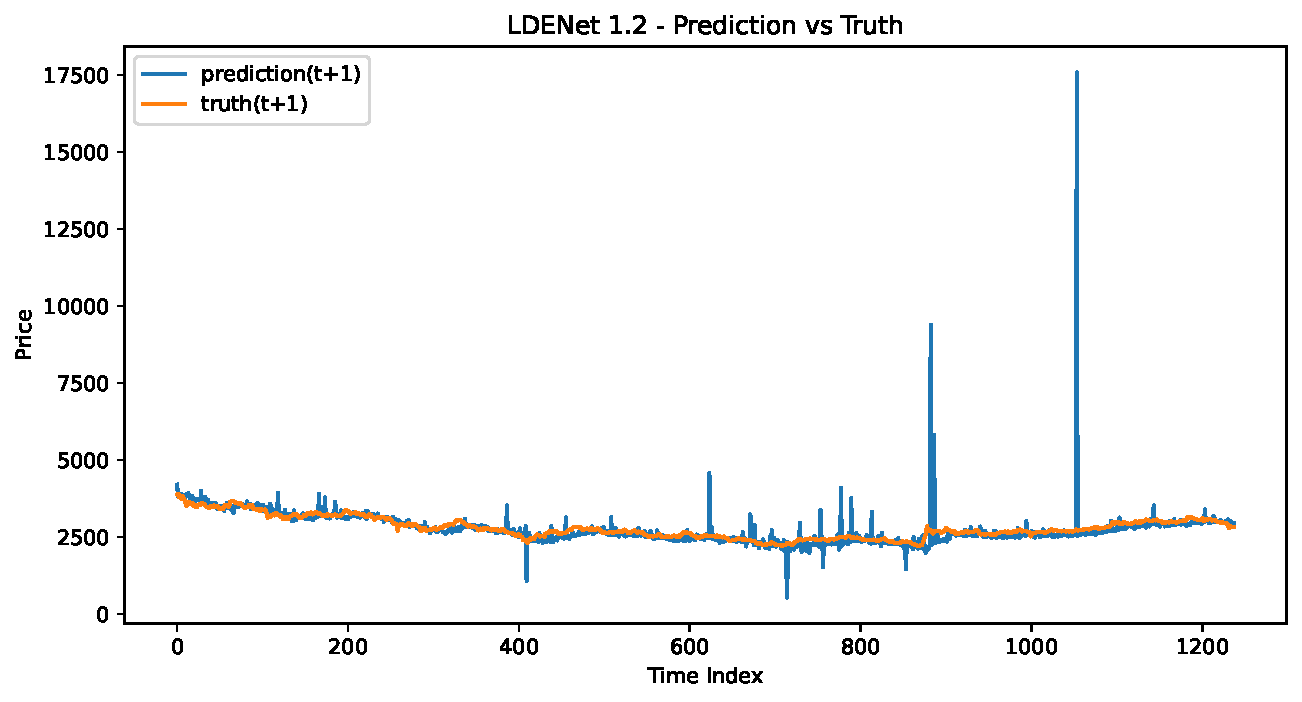
\includegraphics[scale=0.4]{SSE50-LDENet_1.2_PH1_Result}
\caption{SSE50-First Day Forecast Result for LDENet 1.2}
\end{figure}

\begin{figure}[!htbp]
\centering
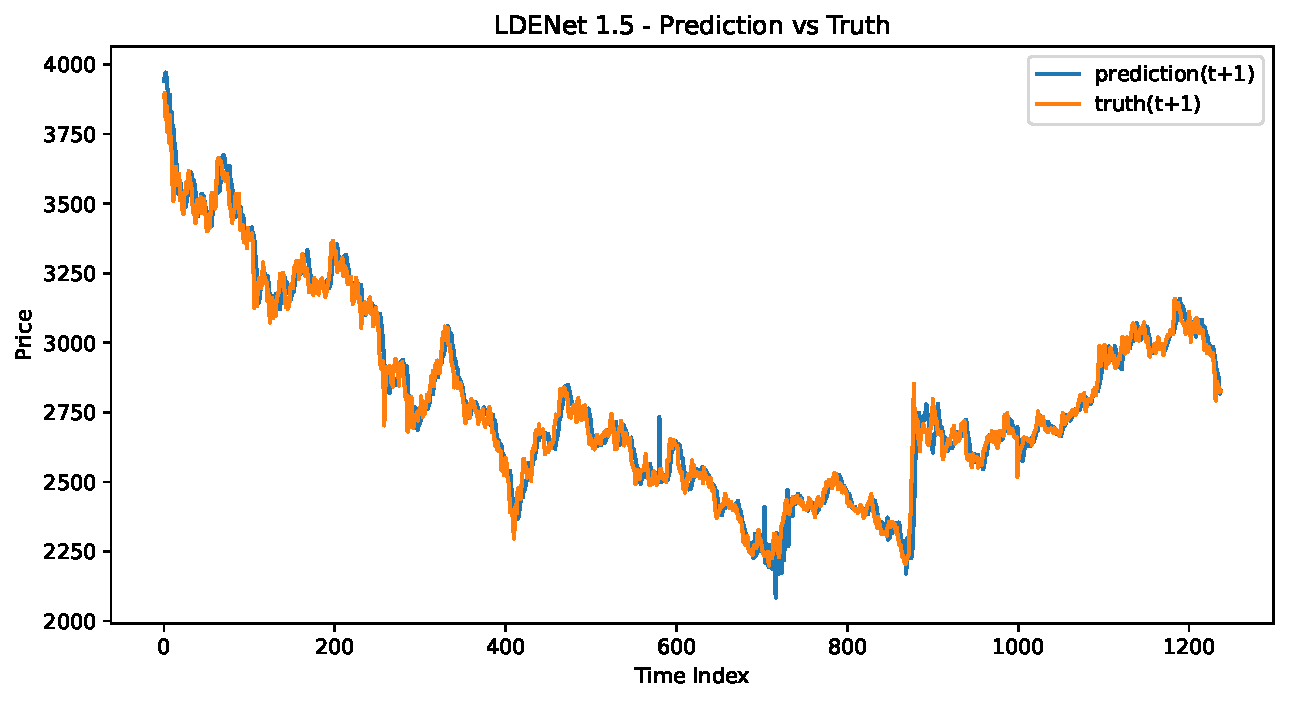
\includegraphics[scale=0.4]{SSE50-LDENet_1.5_PH1_Result}
\caption{SSE50-First Day Forecast Result for LDENet 1.5}
\end{figure}

\begin{figure}[!htbp]
\centering
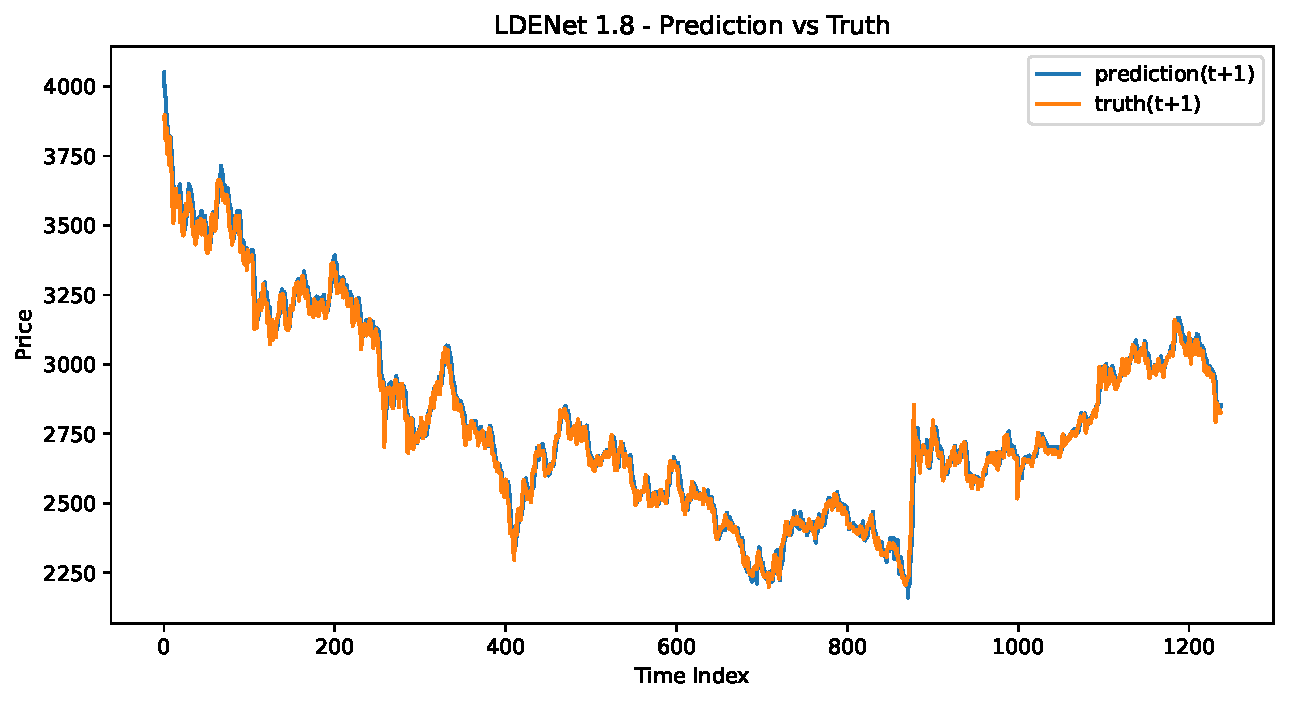
\includegraphics[scale=0.4]{SSE50-LDENet_1.8_PH1_Result}
\caption{SSE50-First Day Forecast Result for LDENet 1.8}
\end{figure}

\newpage

\begin{figure}[!htbp]
\centering
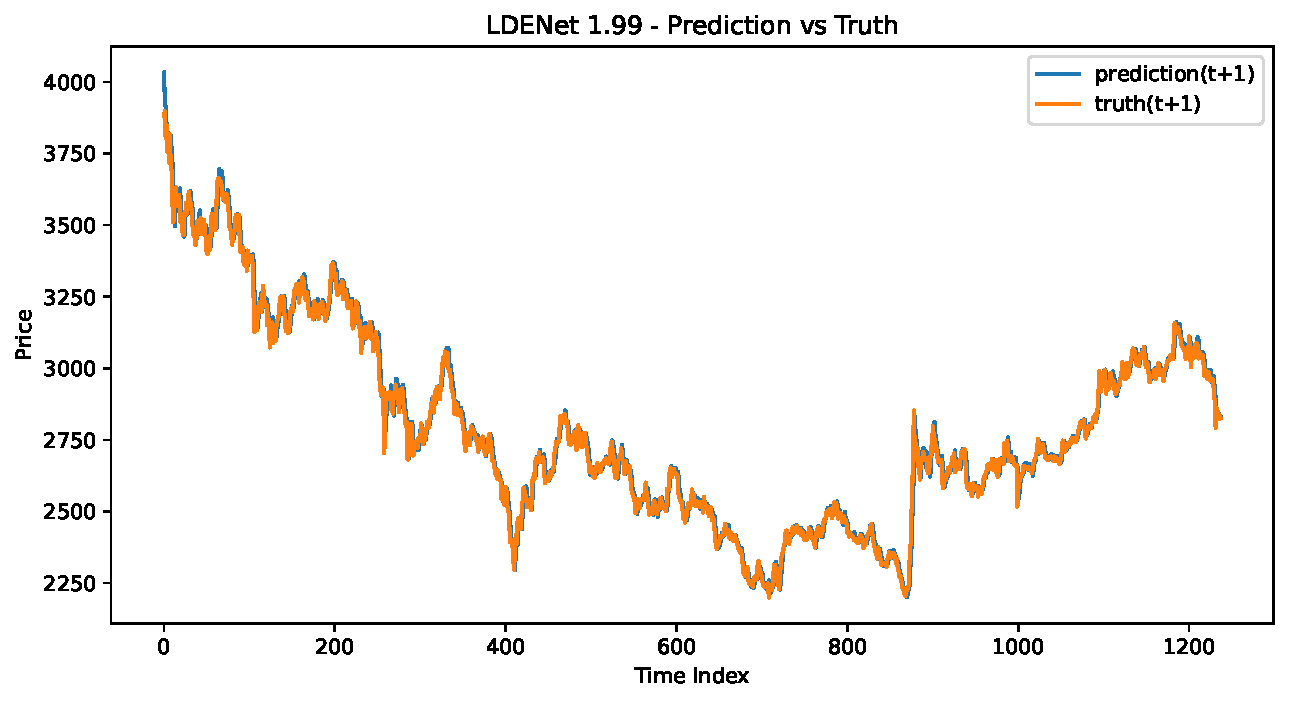
\includegraphics[scale=0.4]{SSE50-LDENet_1.99_PH1_Result}
\caption{SSE50-First Day Forecast Result for LDENet 1.99}
\end{figure}

\begin{table}[!htbp]
\def\arraystretch{1.5}

\begin{center}
\begin{tabular}{>{\centering}m{3cm}>{\centering}m{2cm}>{\centering}m{2cm}>{\centering}m{2cm}>{\centering}m{2cm}>{\centering\arraybackslash}m{2cm}}

\hline

Data & Value of $\alpha$ & MSE$(t+1)$ & MSE$(t+3)$ & MSE$(t+7)$ & MSE$(t+14)$ \\

\hline
\hline

\multirow{4}{*}{SSE50 Index} & $1.2$ & $0.56702$ & $0.61797$ & $1.80748$ & $1.90498$ \\

& $1.5$ & $0.00718$ & $0.00896$ & $0.01834$ & $0.02733$ \\

& $1.8$ & $0.00362$ & $0.00381$ & $0.01481$ & $0.02721$ \\

& \ghl{$1.99$} & $\mathbf{0.00271}$ & $\mathbf{0.00302}$ & $\mathbf{0.01443}$ & $\mathbf{0.02509}$ \\

\hline
\end{tabular}
\end{center}
\caption{Forecast Results for Different $\alpha$}
\label{Results for Different alpha}
\end{table}

From Table (\ref{Results for Different alpha}), it can be seen that the value of $\alpha$ has a certain effect on the prediction of the model. The greater the data fluctuation, the better a smaller $\alpha$ value; this directly corresponds to the fact that Lévy motion with smaller $\alpha$ produce greater jumps. For SSE50 Index value, LDE-Net with $\alpha = 1.99$ gives best predictive accuracy.

\newpage

\subsection{Effect of Forecasting Days on Prediction Accuracy}

The accuracy over prediction days is also investigated and it is found that prediction error is an increasing function of prediction horizon, as the length of forecasting days increase, so does the prediction error. This behaviour is consistent throughout all choices of $\alpha$ as established in Table (\ref{Results for Different alpha}).

\begin{figure}[!htbp]
\centering
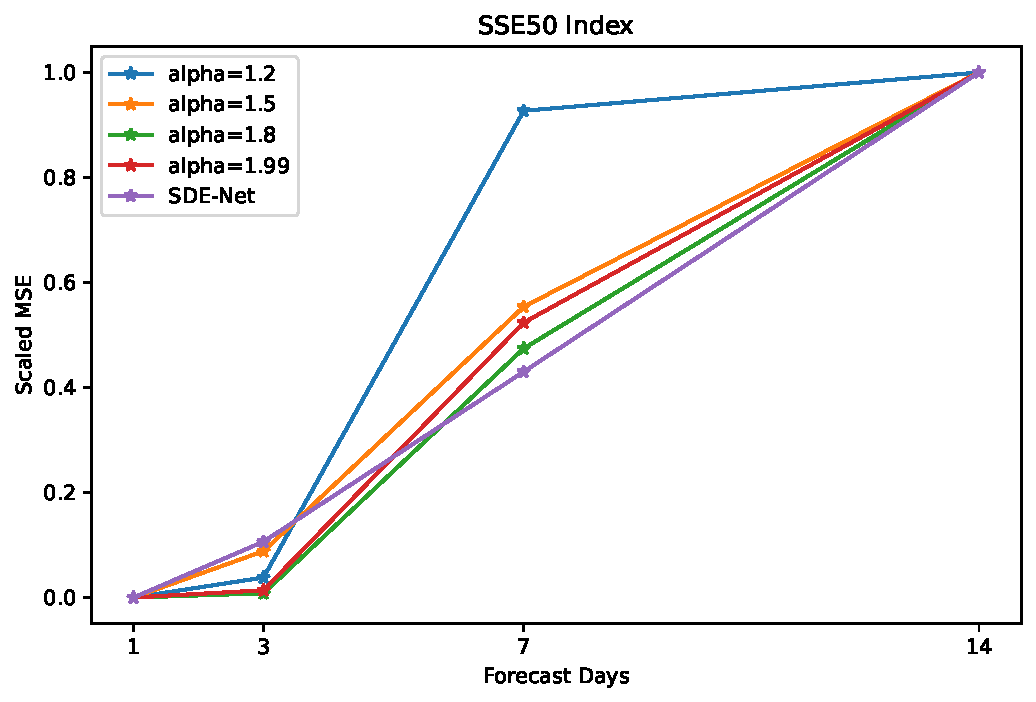
\includegraphics[scale=0.6]{Different_Prediction_Horizons_Different_Alpha}
\caption{Forecast Results for Different Prediction Horizons}
\end{figure}

For NIFTY50, SDE-Net with Brownian Motion gives best predictive performance, while for SSE50, LDE-Net with $\alpha = 1.99$ performs the best in future predictions.

\begin{table}[!htbp]
\def\arraystretch{1.5}

\begin{center}
\begin{tabular}{>{\centering}m{3cm}>{\centering}m{4cm}>{\centering}m{2cm}>{\centering}m{2cm}>{\centering}m{2cm}>{\centering\arraybackslash}m{2cm}}

\hline

Data & Model & MSE$(t+1)$ & MSE$(t+3)$ & MSE$(t+7)$ & MSE$(t+14)$ \\

\hline
\hline

\multirow{2}{*}{NIFTY50 Index} & \ghl{SDE-Net} & $0.00598$ & $0.01635$ & $0.03515$ & $0.30617$ \\

& LDE-Net $(\alpha = 1.99)$ & $0.01238$ & $0.01512$ & $0.03962$ & $0.30149$ \\

\hline
\hline

\multirow{2}{*}{SSE50 Index} & SDE-Net & $0.00333$ & $0.00646$ & $0.01597$ & $0.03272$ \\

& \ghl{LDE-Net $(\alpha = 1.99)$} & $0.00271$ & $0.00302$ & $0.01443$ & $0.02509$ \\

\hline
\end{tabular}
\end{center}
\caption{Prediction Error over Forecasting Days}
\end{table}
\clearpage
\chapter{Conclusion and Future Work}

In this study, we work with a collection of stochastic differential neural networks equipped with Gaussian and Non-Gaussian noise. Brownian motion induced SDEs work fine for data-sets with smoothers fluctuations. On the other hand, special properties of $\alpha-$stable Lévy motion induced SDEs help us to capture large fluctuations and uncertainty in a better way. 

For different prediction horizons, predictive accuracy degrades whatever the model specification we use. 

The model LDE-Net with suitable $\alpha$ is more suitable for predicting time series data that fluctuates with high volatility, as $\alpha$-stable Lévy motion can better capture the training data trend with epistemic jumps.

This leaves us with plenty of future scope of work, a few might be optimal delay time, optimal choice of embedding dimension or a general procedure to obtain optimal $\alpha$. Depending on the objective, different loss functions can also be employed for a better measurement of predictive error. Works can also be done to improve long-term predictive performance. Thus, stochastic differential equations equipped with neural networks propose a very promising framework for data with high volatility.
\clearpage


\printbibliography[heading=bibintoc]
% Comment the following line if you don't want to print
% all the citations in the bibliography file
\nocite{*}


\end{document}
